\chapter{Sprint 1}
\label{chap:S1}
In this sprint, the focus was on learning the tools and languages that are required, finishing the analysis and system requirements, and having a good base for the implementation team to continue work on in sprint 2.

\section{Sprint Plan}
\label{sec:S1Planning}
The group decided that this sprint would be focused on learning the tools and languages that were needed to complete this project, so that we could shift our focus to implementation in the next sprint. \\
\indent When the sprint was finished, analysis had been completed, the system requirements were ready, and we had a good base to make the next sprint a focused implementation sprint. The implementation for this sprint focused on adding photo search to the demo, including sorting and tags, and the implementation lead started considering how to split up later tasks.

\section{Duration and Workload}
\label{sec:S1DurationWorkload}
At the first meeting this sprint we agreed to split the sprints into shorter ones, each lasting one week. \\

\begin{minipage}{\linewidth}
\centering
\setlength{\tabcolsep}{22pt}
\textbf{Sprint 1:} 
\smallskip
\rowcolors{1}{blue!20}{blue!10}
\begin{tabular}{ |l l| }
	\hline
	\it{Duration} & 1 week \\
	\it{Start} & September 15th. \\
	\it{End} & September 21st. \\
	\it{Workload} & Hours spent by the entire group on Sprint 2. \\
	\it{Goal} & 20 - 25 hours per person \\
	\hline
\end{tabular}
\end{minipage}
%
\bigskip
%
\begin{minipage}{\linewidth}
\setlength{\tabcolsep}{25pt}
\centering
\rowcolors{1}{blue!20}{blue!10}
\begin{tabular}{ |l|l| }
	\hline
	\multicolumn{2}{|c|}{\cellcolor{gray!25} Workload} \\
	\hline
	\it{Analysis} & 11 hrs\\
	\it{System requirements} & 5 hrs\\
	\it{Development} & 22 hrs\\
	\it{Testing} & 2 hrs\\
	\it{Learning} & 22 hrs\\
	\it{Documentation} & 8 hrs\\
	\it{Project Management and Meetings} & 58 hrs\\
	\hline
	\textbf{\textit{Total Workload}} & 128 hrs\\
	\hline
\end{tabular}
%Caption here
\captionof{table}{Workload of Sprint 1. \label{tab:S1Workload}} 
\end{minipage}

\bigskip

\subparagraph{} 
The goal for the group was to work 20 - 25 hours each every week. We reached approximately 18 hours each, which means we have some room for improvement. We discussed this at a meeting after the sprint, and it became clear that once people finished assigned tasks, they did not have a clear idea of what to do next, and that they were uncomfortable just deciding on a task to do. This meant that creating a backlog became a priority, so that people would have an easier time finding tasks. This will be looked at further in section \ref{sec:S1Retrospective}.

\section{Backlog}
\label{sec:S1Backlog}
At this point in the project, we had not yet created a backlog to select tasks from. Because of this, we use this section to detail what tasks we planned to do, and for most tasks there was no accuracy to extimated time beyond one week. \\
\begin{minipage}{\linewidth}
\setlength{\tabcolsep}{12pt}
\centering
\rowcolors{1}{blue!20}{blue!10}
\begin{tabular}{|p{1cm}|p{4cm}|p{2cm}|p{2cm}|}
\hline
\cellcolor{gray!25} ID & \cellcolor{gray!25} Description & \cellcolor{gray!25} Estimated Time & \cellcolor{gray!25} Actual Time \\
\hline
N/A & \it{Adding the ability to search for photos on a location-interest coordinate system.} & N/A & 21 hours \\
N/A & \it{The system requirements still have to be finished} & N/A & 5 hours \\
N/A & \it{System development tasks need to be split up and time for each of these estimated} & N/A & 5 hours \\
N/A & \it{Finishing the market analysis} & N/A & 11 hours \\
\hline
\end{tabular}
\captionof{table}{Backlog for sprint 1. \label{tab:S1Backlog}} 
\end{minipage}

\section{Analysis}
\label{sec:S1Analysis}
Two members of the team spent some time doing market analysis for the project. This had mostly been done during the planning phase, but they finished it up at the beginning of this sprint. This work focused on competitor analysis and revenue generation. Since we knew that revenue generation was not a priority considering the vision for the project, we decided to stop the analysis at a cursory glance at different possibilities. To get an overview of this analysis, see section \ref{sec:PrelimMarket}, the cursory ideas for revenue possibilities are found in \ref{subsec:PrelimMarketRevenue}.

\paragraph{} Since ASpaces would be focused on teenagers and youth, a discussion was started on whether as diverse an age group as 10-17 might need events and interests tailored to smaller age groups, and therefore exclusive to those age groups. This might be particularly interesting to keep older kids from pestering the younger ones. In the end, since we decided that this would be completely open to view for anyone, even without a user, it would be difficult for us to implement this feature without also compromising this functionality. Another objection was that it might not do much good, since we would have no reliable way of ensuring a person's age was correct without huge amounts of administration.

\paragraph{} The analysis also brought up the idea of one to one messaging. Practically all other social media had the ability to message another user directly, either as a chat or as a "mail" message. We quickly agreed that we did not think this page would outcompete Facebook or Instagram, so a chat system one to one would not be something we needed. Mail messaging was considered more feasible, but we decided it would not be a focus, and that the prototype would not need it. We also considered the ability to place chat rooms on the map. In the end this was scrapped in favour of possibly adding discussions (essentially a comment placed on the map with an accompanying title).

\section{Implementation}
\label{sec:S1Implementation}
In this sprint, most of the implementation team focused on learning or relearning JavaScript, PHP, and CSS. The technical lead was the only person working on the system. He spent his time developing a basic system for searching for photos on a location-interest coordinate system, in order to get informed customer feedback about such a system at the earliest opportunity. After finishing that task, he started looking at how to split up later tasks in preparation for creating a backlog next sprint.

\begin{figure}[ht!]
\centering
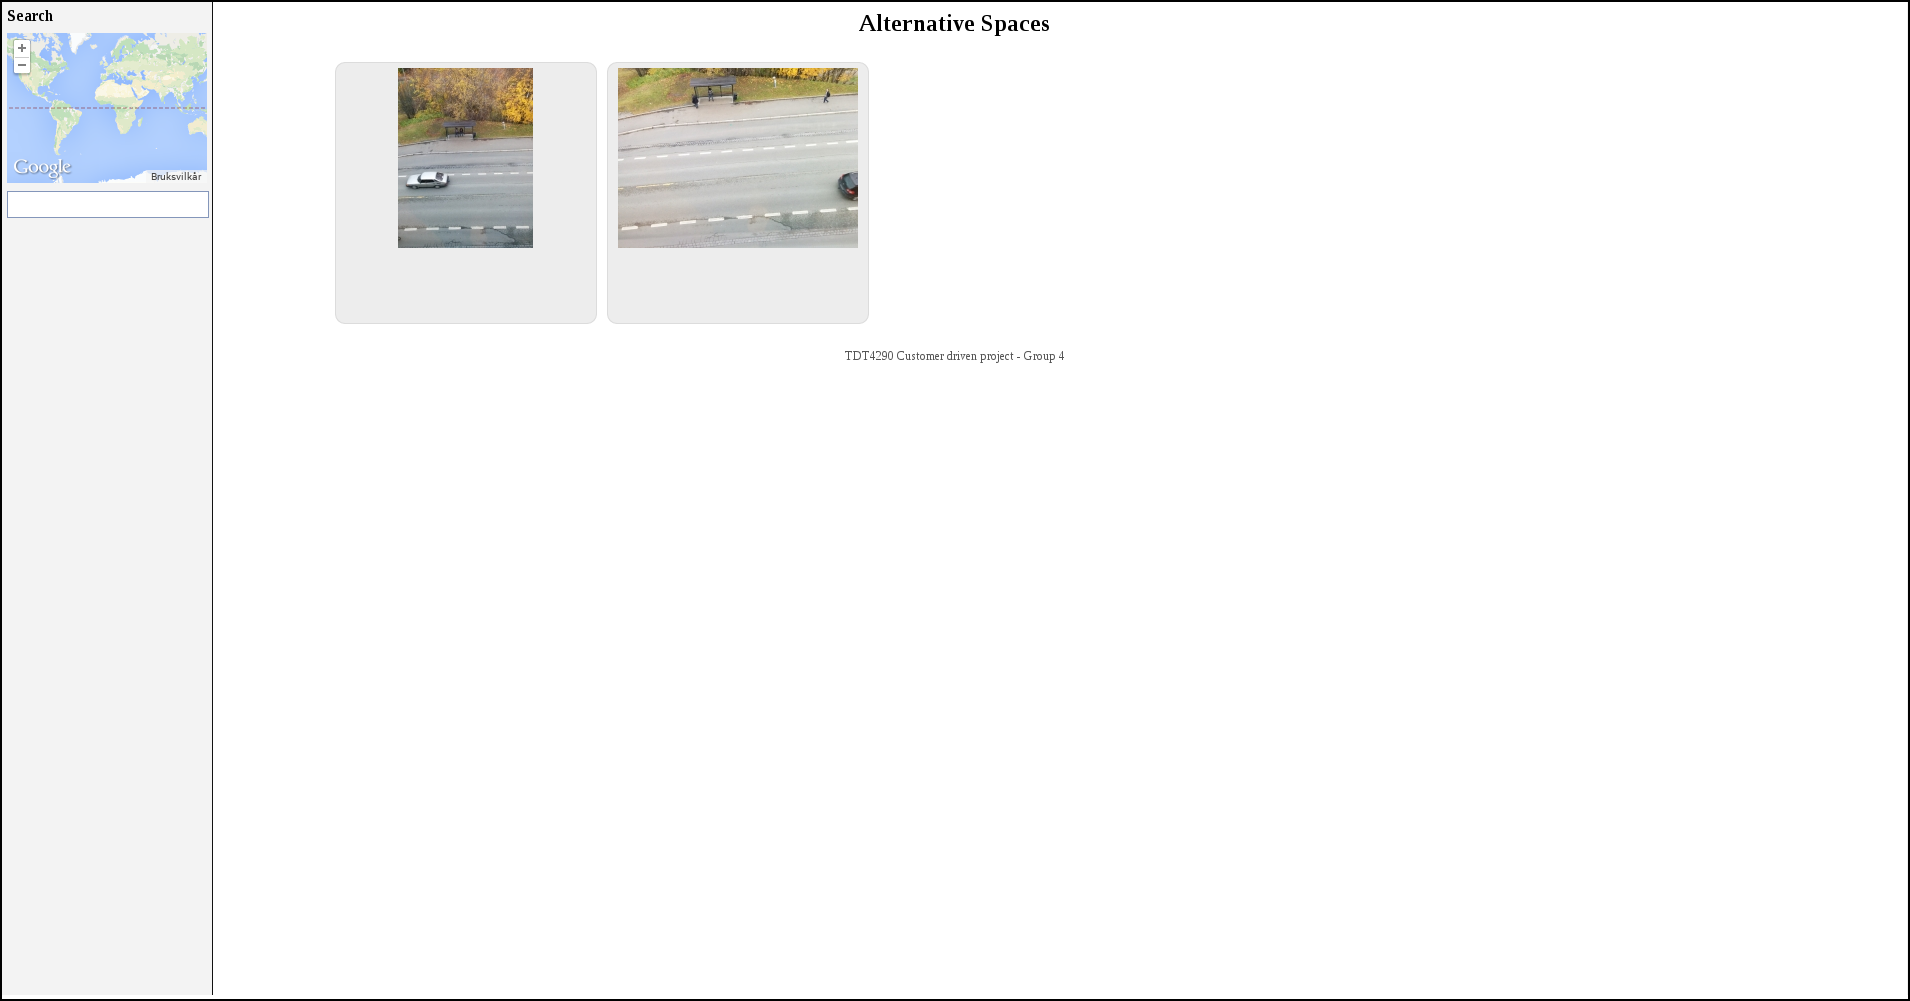
\includegraphics[width=\linewidth]{./img/webpage/22Sep/Photos22Sep}
\caption{The Photos page after Sprint 1. \label{fig:Photos22Sep}}
\end{figure}

\subsection*{Photo Search}
As mentioned the photo search idea was to have the ability to search for pictures on based on location and interests, and the technical lead spent most of his time this sprint developing and testing the initial part of this system. The system would consist of finding photos taken within the boundaries of a map concerning chosen interests. These would be sorted by some as yet undetermined rating system, to be added in a later sprint.
\paragraph*{} The initial results were promising, as can be seen in figure \ref{fig:Photos22Sep}, although we found that there was too much unused space. We decided to spend time in a future sprint to come up with different designs for the page.

\section{Sprint Retrospective}
\label{sec:S1Retrospective}

\subsection{Start Doing}
\label{subsec:S1RetrospectiveStart}

\begin{itemize}
  \item Write better work summaries.
  \item Be proactive in asking for tasks.
  \item Create product backlog immediately.
  \item Create sprint backlogs each sprint.
  \item Ask questions.
\end{itemize}

\subsection{Stop Doing}
\label{subsec:S1RetrospectiveStop}

\begin{itemize}
  \item Working without input.
\end{itemize}

\subsection{Continue Doing}
\label{subsec:S1RetrospectiveContinue}

\begin{itemize}
  \item Learning required skills for the project
  \item Updating your hours.
  \item Keep documents up to standard.
\end{itemize}

\subsection{Group Dynamics}
\label{subsec:S1RetrospectiveGroupDynamics}
As mentioned in \ref{sec:S1DurationWorkload}, the group managed an average of 18 hours of work per member during the sprint. Although being a good beginning, it was not as many work hours as we had hoped for and set as our goal. When we discussed it, we found that the vague idea of learning the skills needed, as well as the lack of a good overview of required tasks meant that people did not know what they needed to do. Because group members lacked experience working with Scrum,  it took time to get into how things were done. We decided to immediately create a backlog to get more efficiency.

\paragraph{} At the beginning of this sprint we realized that the originally envisioned two sprints were too few, and it was suggested to split the original first sprint into fewer, shorter sprints. In the end we decided on one week sprints being the goal, making this sprint last until next monday, to give the group a better ability to review progress.

\begin{figure}[ht!]
  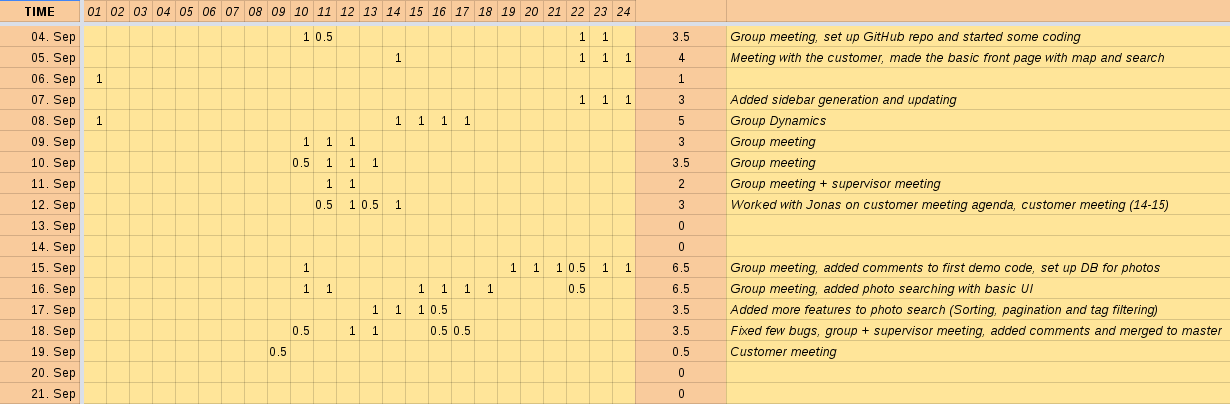
\includegraphics[width=\linewidth]{./img/WorkSheetExample}
  \caption{Example of a well made work summary}
\end{figure}


\paragraph{} To make sure we had a good overview of work done, it was reiterated that keeping our work hours updated in the group's work summary document on Google Drive was very important. Members were not always good at updating it on time, and since knowing the specifics of what had been done was important for later documentation in the report, updating it later was problematic. People often wrote work summaries that were very lacking in detail.

\subsection{Customer Feedback}
\label{subsec:S1RetrospectiveCustomerFeedback}
The customer were very pleased with our work on the Photo Search, and gave us only positive feedback to our ideas. They deferred to our judgement regarding the technology, since they have very little experience regarding what is and is not possible. Beyond showing them the demo and receiving some feedback, and a report on our market analysis, the meeting focused on discussion of a workshop where we could receive more direct user feedback. The date had not yet been set, but they wanted us to prepare for it, and would give us more information at the next meeting.